%======================================================%
%   Beamer Presentation
%   LaTeX Template
%   compile using PDFTeXify, PDFLaTeX or XeLaTeX
%======================================================%

%--------------------------------------------------------------------------------
%   PACKAGES AND THEMES
%--------------------------------------------------------------------------------

\documentclass[notheorems,10pt,compress]{beamer}

\mode<presentation>{
	
	%------- Beamer theme ------
	\usetheme{Madrid}
	%\usetheme{Boadilla}
	%\usetheme{Frankfurt}
	%\usetheme{Warsaw}
	%\usetheme{CambridgeUS}
	%\usetheme{Montpellier}
	
	%------- Color theme ------
	\usecolortheme{rose}
	%\usecolortheme{orchid}
	%\usecolortheme{lily}
	%\usecolortheme{whale}
	%\usecolortheme{dolphin}
	%\usecolortheme{seahorse}
	
	%\usetheme{boxes}
	%\setbeamercovered{transparent}
	%\usefonttheme[onlymath]{serif}
	\usefonttheme{serif}
	\usefonttheme{professionalfonts}
	
	
	%\setbeamertemplate{headline}{}
	%\setbeamertemplate{footline}{}
	\setbeamertemplate{blocks}[rounded][shadow=true]
	\setbeamertemplate{navigation symbols}{}
	%\setbeamertemplate{itemize items}[square]  % ball, circle, square
	\setbeamertemplate{enumerate items}[default]
	%\setbeamertemplate{section in toc}[square]
	
}

%--------- 宏包  ----------
\usepackage[UTF8,noindent]{ctex}
%\usepackage[english]{babel}
\usepackage{amsmath,amssymb,version}
\usepackage{graphicx,fancybox,mathrsfs,multirow}
\usepackage{booktabs}
\usepackage{epsfig,epstopdf}
\usepackage{url,hyperref}
\usepackage{tabularx,array,makecell}
\usepackage{color,xcolor}
\usepackage{cases}
\usepackage{mathtools}
\usepackage{tikz}
\usepackage{indentfirst}
%---------- 定义行距 ----------
\renewcommand{\baselinestretch}{1.15}

%---------- 定义表格新命令 ----------
\newcolumntype{P}[1]{>{\centering \arraybackslash}p{#1}}
\newcolumntype{L}{>{\quad}X}
\newcolumntype{C}{>{\centering \arraybackslash}X}
\newcolumntype{R}{>{\raggedright \arraybackslash}X}


\newcommand{\RR}{\ensuremath{\mathbb{R}}}
\newcommand{\EE}{\mathbb{E}}

%---------- 设置字体  ----------
\setbeamerfont{normal text}{family=\rmfamily}
\setbeamerfont{frametitle}{family=\rmfamily}
\setbeamerfont{title}{family=\rmfamily}
\setbeamerfont{subtitle}{family=\rmfamily}
\setbeamerfont{institute}{family=\kaishu}
\setbeamerfont{author}{family=\kaishu}
%\setbeamerfont{date}{family=\rmfamily}
\setbeamerfont{footline}{family=\kaishu}
\setbeamerfont{section in toc}{family=\rmfamily}
\setbeamerfont{subsection in toc}{family=\rmfamily}
\AtBeginDocument{\usebeamerfont{normal text}}

\setbeamertemplate{caption}[numbered]
\numberwithin{figure}{section}
\numberwithin{table}{section}
\numberwithin{equation}{section}

%---------- 定理设置  --------------
\setbeamertemplate{theorems}[numbered]
%\newtheorem{theorem}{Theorem}
\newtheorem{theorem}{定理}
\numberwithin{theorem}{section}
%\newtheorem{definition}{Definition}
\newtheorem{definition}{定义}
\numberwithin{definition}{section}
%\newtheorem{lemma}{Lemma}
\newtheorem{lemma}{引理}
\numberwithin{lemma}{section}
%\newtheorem{proposition}{Proposition}
\newtheorem{proposition}{命题}
\numberwithin{proposition}{section}
%\newtheorem{corollary}{Corollary}
\newtheorem{corollary}{推论}
\numberwithin{corollary}{section}
\theoremstyle{example}
%\newtheorem{example}{Example}
\newtheorem{example}{例}
%\numberwithin{example}{section}
\renewenvironment{proof}[1][证明]{\textbf{#1}:~~}{\qed\par}
\newenvironment{solution}{\par\noindent\textbf{解}:~~}{\par}

%---------- 调节公式的间距 ----------
%\AtBeginDocument{
	%	\setlength{\abovedisplayskip}{4pt plus 1pt minus 1pt}
	%	\setlength{\belowdisplayskip}{4pt plus 1pt minus 1pt}
	%	\setlength{\abovedisplayshortskip}{2pt}
	%	\setlength{\belowdisplayshortskip}{2pt}
	%	\setlength{\arraycolsep}{2pt}
	%}


\makeatletter
\newcommand\HUGE{\@setfontsize\Huge{36}{42}}
\makeatother

\def\a{\alpha}
\def\e{\varepsilon} \def\z{\zeta} \def\y{\eta} \def\o{\theta}
\def\vo{\vartheta} \def\k{\kappa} \def\l{\lambda} \def\m{\mu} \def\n{\nu}
%\AtBeginSection[]{
	%\begin{frame}
	%  \frametitle{Outline} %\small
	%  \vskip -5pt
	%  \hspace*{1.5em}
	%  \parbox[t]{.95\textwidth}{
		%  \begin{minipage}[c][0.6\textheight]{\textwidth}
			%  \tableofcontents[currentsection,currentsubsection,subsectionstyle=show/show/shaded]
			%  \end{minipage}
		%  }
	%  \addtocounter{framenumber}{-1}
	%\end{frame}
	%}


%---------- 自定义命令 ----------
\newcommand{\red}[1]{\textcolor{red}{#1}}
\newcommand{\blue}[1]{\textcolor{blue}{#1}}


%--------------------------------------------------------------------------------
%	TITLE PAGE
%--------------------------------------------------------------------------------

\title[时间变换随机微分方程的Milstein型方法]{一类高非线性非自治时间变换随机微分方程的Milstein型方法}

\author[吴若雪]
{
	%答辩人:吴若雪~~ \vskip 3mm
	报告人:吴若雪~~ \vskip 3mm
	专业:计算数学 \vskip 3mm
	指导教师:刘暐 ~ 副研究员 \vskip 3mm
	研究方向:随机微分方程数值解
}
%\author[姓名]{报告人姓名}

\institute[上海师范大学]{}
%\institute[学校名称]{\normalsize 学校名称}

\date[2023.9.27]{2023.9.27}

\graphicspath{{./figures/}}

\begin{document}
	
	
	\begin{frame}
		\titlepage
	\end{frame}
	
	\begin{frame}
		\frametitle{Outline}
		\vskip -5.6pt
		\hspace*{1.5em}
		\parbox[t]{.95\textwidth}{
			\begin{minipage}[c][0.6\textheight]{\textwidth}
				\tableofcontents
			\end{minipage}
		}
	\end{frame}
	
	%--------------------------------------------------------------------------------
	%	PRESENTATION SLIDES
	%--------------------------------------------------------------------------------
	\section{研究背景与意义}
    
\begin{frame}
\frametitle{1.研究背景与意义\\\zihao{-4} 1.1 研究背景}
		
            \begin{itemize}
                \setlength{\itemsep}{10pt}
      \item 时变随机过程和时变随机微分方程(SDEs)作为描述亚扩散过程重要工具之一, 在众多领域发挥着重要作用. 包括:金融模型、生物化学等领域\footnote{Marcin Magdziarz, Sebastian Orzel, and Aleksander Weron. Option pricing in subdiff-\\
          usive Bachelier model. J.Stat. Phys., 145(1):187–203, 2011.}.
            
      \item 传统的随机微分方程数值方法包括Euler型方法、Milstein型方法、Runge-
      Kutta方法等. 但当随机微分方程项出现超线性增长时,经典的方法可能不收敛\footnote{Martin Hutzenthaler, Arnulf Jentzen, and Peter E. Kloeden. Strong and weak diverge-\\
          nce in finite time of Euler’s method for stochastic differential equations with non-globally Lipschitz continuous coefficients. Proc. R. Soc. Lond. Ser. A Math. Phys. Eng. Sci., 467
          (2130):1563–1576, 2011.}.
	
            
       \end{itemize}
	\end{frame}

\begin{frame}		
\frametitle{\zihao{-4} 1.2 研究意义}

            \begin{itemize}
           \setlength{\itemsep}{10pt}
            \item  具有超线性系数的经典布朗运动驱动的随机微分方程, 大量工作利用隐式方法进行研究, 隐式方法计算复杂度高、计算效率低.
             \item 时间变换的随机微分方程的真实解解很少能显式地表达出来, 因此其数值逼近尤为重要.
            \item 处理具有超线性增长项的随机微分方程, 截断Euler-Maruyama的强收敛率较低, 构造一种截断Milstein型方法具有重要的研究意义.   
           

       \end{itemize}
\end{frame}


	\section{国内外研究现状}

\begin{frame}
    \frametitle{2.国内外研究现状\\\zihao{-4}}
\quad {\bf 2.1 超线性增长项SDEs的研究}
\vskip 10pt
\setlength{\parindent}{2em} 隐式方法可用于处理具有超线性项的经典布朗运动驱动的随机微分方程.由于显式数值方法结构清晰, 计算复杂度低, 近年来在处理超具有线性项的随机微分方程时常用改进显式方法:
    \begin{itemize}
        \setlength{\itemsep}{10pt}
        \item \blue{ X. Mao(2013) } 研究了向后Euler-Maruyama的强收敛率. 
        \item \blue{J. Gao, H. Liang, S. Ma(2019)} 研究semi-implicit Euler方法的强收敛.
\item \blue{M. Hutzenthaler, A. Jentzen, P.E. Kloeden (2012) } 研究了具有非全局
Lip-\\
schitz条件的SDEs的Tamed Euler方法.
\item \blue{ X. Mao(2015) } 提出利用截断Euler-Maruyama方法去处理具有超线性增长项的SDEs.           
    \end{itemize}
\end{frame}
		
        
        \begin{frame}
            \frametitle{2.国内外研究现状\\\zihao{-4}}
            \quad {\bf 2.2 时变SDEs数值方法的研究}
            \begin{itemize}
                \setlength{\itemsep}{10pt}
         \item \blue{ Ernest Jum, Kei Kobayashi(2016) } 第一篇关于离散格式下时间变换随机微分方程的数值逼近研究. 
          \item \blue{ Sixian Jin, Kei Kobayashi(2019) }  系数满足全局Lipschitz条件下, 研究了时间变换SDEs的EM方法.
    \item \blue{ Sixian Jin, Kei Kobayashi(2021) } 研究时变SDEs的Milstein型方法.
    \item \blue{ Chang-Song Deng and Wei Liu(2020) } SDEs满足超线性增长条件时, 研究了半隐式EM方法.
     \item \blue{Wei Liu, Xuerong Mao, Jingwen Tang, and Yue Wu(2020) }利用对偶原则研究了截断EM方法. 
            \end{itemize}
        \end{frame}
%------------------------------------------------
\section{研究内容与主要工作}
%------------------------------------------------

\begin{frame}
    \frametitle{3.研究内容与主要工作\\\zihao{-4} 3.1 研究内容}
   \setlength{\parindent}{2em}我们考虑一类时间变换随机微分方程(SDEs):
   \begin{block}{}
       \begin{equation*}\label{SDE}
           dY(t) = f(t,Y(t))dE(t) + g(t,Y(t))dW(E(t)),~~Y(0) = Y_0,
       \end{equation*}
   \end{block}
   其中$f$为SDEs的漂移项, $g$为扩散项. 这里$T>0$, $t\in [0,T]$, 对所有 $q > 0$有$\EE |Y_0|^q < \infty$. $f: \RR_+ \times \RR^d \rightarrow \RR^d$ 和 $g: \RR_+ \times \RR^d \rightarrow \RR^{d}$.
\\ 对于上述方程, 我们的\alert{研究内容}如下:
\begin{itemize}
    \setlength{\itemsep}{0.1pt}
    \item 对一类具有超线性增长系数, 且不满足对偶原则的时变SDEs构造Trucated-Milstein数值方法, 并进行收敛性分析;
    \item 通过Matlab编程, 数值验证一维和高维数值例子成立.
\end{itemize}
\end{frame}

\begin{frame}		
    \frametitle{\zihao{-4} 3.2 主要工作}
    %\begin{block}{}
  \hspace{2em}在一类高非线性非自治时变SDEs中,其系数满足以下条件:
  \begin{itemize}
      \setlength{\itemsep}{0.1pt}
      \item  $f$和$g$的空间变量满足超线性增长,
       \begin{eqnarray*}
           &&|f(t,x)-f(t,y)|\vee |g(t,x)-g(t,y)|\vee |Lg(t,x)-Lg(t,y)|\\
           &&\leq C(1+|x|^{\a}+|y|^{\a})|x-y|,
       \end{eqnarray*}   
    \item $f$和$g$的时间变量满足H{\"o}lder连续,
    \begin{eqnarray*}
        &&|f(s,x)-f(t,x)|\leq H_1(1+|x|^{\a+1})(s-t)^{\gamma_{f}},\\
        &&|g(s,x)-g(t,x)|\leq H_2(1+|x|^{\a+1})(s-t)^{\gamma_{g}},
    \end{eqnarray*}
\end{itemize}
\hspace{2em}我们研究时变SDEs的Trucated-Milstein方法强收敛性:
 \begin{block}{}
    \begin{equation*}
           \EE\left( \sup_{0\leq t\leq T}|Y(t)-X(t)|^{\bar{p}}\right)\leq h^{\min\{\gamma_f\bar{p},\gamma_g\bar{p},(1-2\varepsilon)\bar{p}\}}.
    \end{equation*}
\end{block}
\end{frame}
		
            \begin{frame}		
                \frametitle{\zihao{-4} 3.2 主要工作}
        \setlength{\parindent}{2em}本论文研究一类时变SDEs方程的Trucated-Milstein方法的强收敛率, 具体工作如下:
        \vskip 5pt
        \begin{itemize}
            \setlength{\itemsep}{5pt}
            \item 选择合适的截断函数, 构造Trucated-Milstein方法.
            \item 证明真实解和数值解的有界性.
            \item 验证数值解的连续时间关系.
            \item 结合Talay展开、Young不等式、Jensen’s不等式、Gronwall’s不等式、H{\"o}lder不等式等进行收敛性分析.
            \item 利用Matlab编程进行数值模拟, 验证理论结果的正确性.
        \end{itemize}
    \end{frame}
		
     \begin{frame}		
      \frametitle{\zihao{-4} 3.2 主要工作}
       \setlength{\parindent}{2em}本论文通过一维和二维数值算例进行理论验证:
       \vskip 5pt
      \begin{itemize}
          \setlength{\itemsep}{5pt}
            \item 考虑一维时间变换随机微分方程:
             \begin{align*}
                 \left\{
                 \begin{array}{lr}
                     dY(t)=\left([t(1-t)]^{\frac{1}{4}}Y(t)-Y^5(t)\right)dE(t)+\left([t(1-t)]Y^2(t)\right)dW(E(t)),&\\
                     Y(0)=1.&
                 \end{array}
                 \right.
             \end{align*}
         \item 考虑二维时间变换随机微分方程:
         \begin{align*}
             \label{ex2}
             \left\{
             \begin{array}{lr}
                 dx_1(t)=\left([t(1-t)]^{\frac{1}{5}}x_1(t)-x_2^5(t)\right)dE(t)+\left([t(1-t)]^{\frac{1}{2}}x_2^2(t)\right)dW(E(t)),&\\
                 dx_2(t)=\left([t(1-t)]^{\frac{1}{5}}x_2(t)-x_1^5(t)\right)dE(t)+\left([t(1-t)]^{\frac{1}{1}}x_1^2(t)\right)dW(E(t)).&
             \end{array}
             \right.
         \end{align*}
       \end{itemize}
        \end{frame}
    
    
\begin{frame}		
    \frametitle{\zihao{-4} 3.2 主要工作}
         一维和二维时间变换随机微分方程的Trucated-Milstein方法数值结果:

\begin{figure}[!htp]
    \begin{minipage}[h]{0.48\linewidth}
        \centering
        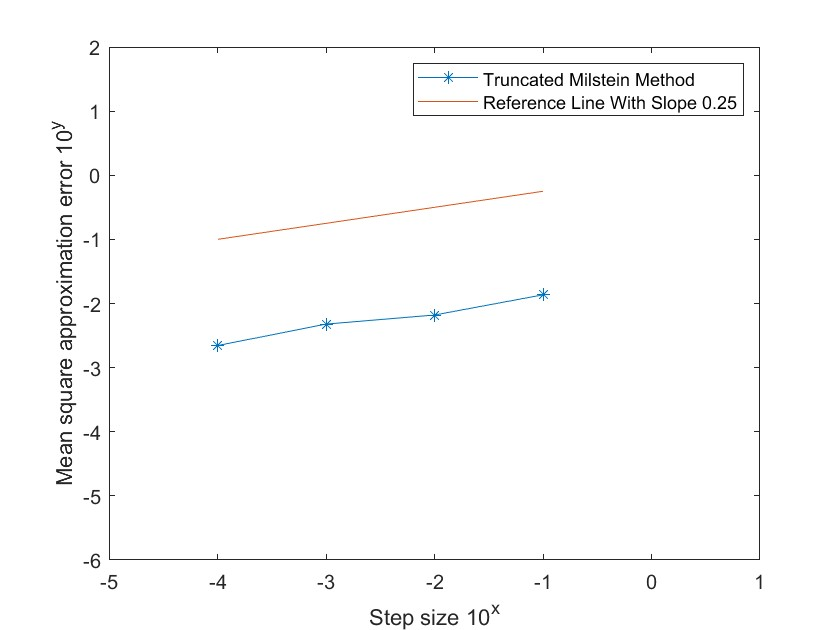
\includegraphics[width=0.9\linewidth]{image1}
        \caption{一维SDE强收敛率为0.25}
        \label{image1}
    \end{minipage}
    \begin{minipage}[h]{0.48\linewidth}
        \centering
        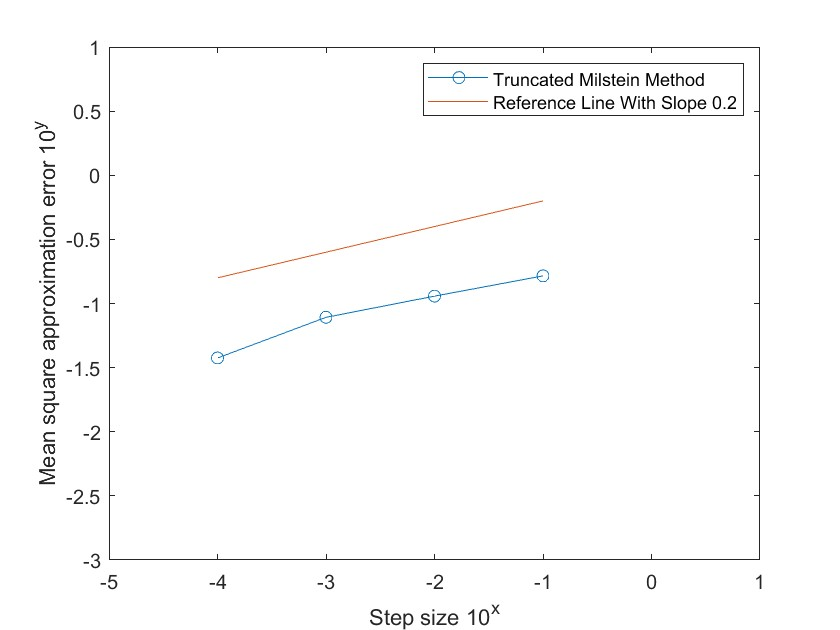
\includegraphics[width=0.9\linewidth]{image2}%width=\textwidth
        \caption{二维SDE强收敛率为0.2}
        \label{image2}
    \end{minipage}
\end{figure}
\end{frame}
		%------------------------------------------------
		\section{论文创新点与问题}
		

    	\begin{frame}{论文创新点与问题}
    \frametitle{4.论文创新点与问题\\\zihao{-4}}
    \begin{block}{}
        \vskip 6pt
        \begin{itemize}
            \setlength{\itemsep}{6pt}
            \item 我们考虑数值方法具有更高的收敛阶, 提出了一种采用截断技术抑制超线性项的Milstein型方法.
            \item 本文研究的时间变换随机微分方程不满足对偶原理, 并在非自治情况下进行研究.
             \item 在一维和多维的时变SDEs数值例子上进行了模拟, 然而将数值方法应用于多水平蒙特卡罗方法的期权选择等研究中,由于步长选择的不同,其研究受到一定的限制.
        \end{itemize}
    \end{block}
\end{frame}
		
		\section{论文进度安排及预期成果}
		

    
\begin{frame}{论文进度安排及预期成果}
    \frametitle{5.论文进度安排及预期成果\\\zihao{-4} 5.1 进度安排}
\begin{table}[htp!]
\centering
\renewcommand\arraystretch{1} %定义表格高度
% PLCR前面已经定义
\begin{tabularx}{0.98\textwidth}{||P{2.8cm}|C||}
\Xhline{2\arrayrulewidth}
起止时间       &  论文进度安排\\
\hline
2023.2 -2023.3    &  论文定题,收集、阅读并整理相关图书、文献\\
\hline
2023.4 -2023.7    &  完成时间变换SDEs截断方法的构造,进行强收敛率推导、数值模拟\\
\hline
2023.8 -2023.9    &  论文撰写、修改、完成开题报告\\
\hline
2023.10 -2023.11    & 推导过程和数值模拟总结,进行排版、整理,初步完成论文初稿\\
\hline
2023.12 - 2024.1    &  毕业论文预答辩\\
\hline
2024.2 -2024.4    &  补充、完善论文,论文定稿\\
\hline
2024.5    &  毕业论文答辩\\
\Xhline{2\arrayrulewidth}
\end{tabularx}
\end{table}

\end{frame}

\begin{frame}
    \frametitle{\zihao{-4} 5.2 预期成果}
    \begin{block}{}
        \hspace{2em}本论文研究一类高非线性非自治时间变换SDEs的Trucated-Milstein方法, 其\alert{预期成果}如下:
        \vskip 6pt
        \begin{itemize}
            \setlength{\itemsep}{6pt}
            \item 利用截断思想构造处理超线性增长项的Trucated-Milstein方法.
            \item 验证数值方法的强收敛性, 并给出强收敛率.
            \item 给出时变SDEs的Trucated-Milstein方法的实现代码, 通过一维和高维数值算例对理论结果进行验证, 形成研究论文.
        \end{itemize}
    \end{block}
\end{frame}

	%-----------------------------------------------
\section{主要参考文献}


\begin{frame}
    \frametitle{6.主要参考文献\\\zihao{-4}}
    
    
    \textcolor[rgb]{0.00,0.00,1.00}{对超线性增长项SDEs的研究:}
    \begin{itemize}
        
        \item Martin Hutzenthaler, Arnulf Jentzen, and Peter E. Kloeden. Strong and weak divergence in finite time of Euler’s method for stochastic differential equations with non-globally Lipschitz continuous coefficients. Proc. R. Soc. Lond. Ser. A Math. Phys. Eng. Sci., 467(2130):1563–1576, 2011.
        \item Xue-Rong Mao. The truncated euler–maruyama method for stochastic differentia lequations.Comput. Appl. Math.,  290:370–384. 2015.
        \item Qian Guo, Wei Liu, Xue-Rong Mao and  Rong-Xian Yue. The truncated milstein method for stochastic differential equations with commutative noise. Journal of Computational and Applied Mathematics., 338:298 – 310. 2018.
        
        
    \end{itemize}
\end{frame}


\begin{frame}
    \frametitle{6.主要参考文献\\\zihao{-4}}
    \textcolor[rgb]{0.00,0.00,1.00}{对时变SDEs数值方法的研究:}
    \begin{itemize}
        \item Ernest Jum and Kei Kobayashi. A strong and weak approximation scheme for stochastic differential equations driven by a time-changed Brownian motion. Probab. Math. Statist., 36(2):201–220, 2016.
        \item Sixian Jin and Kei Kobayashi. Strong approximation of time-changed stochastic differential equations involving drifts with random and non-random integrators. BIT, 61(3):829–857, 2021.
        \item Chang-Song Deng and Wei Liu. Semi-implicit Euler-Maruyama method for non-linear time-changed stochastic differential equations. BIT, 60(4):1133–1151, 2020.
        
    \end{itemize}
\end{frame}

		

\begin{frame}{}
    \vskip 1cm
    \begin{center}
        \sffamily
        \HUGE{\textcolor[RGB]{1,8,9}{\zihao{-1}请各位老师批评指正!\\[1mm]谢谢!}}
        %\includegraphics[width=\textwidth]{Thankyou2}
    \end{center}
\end{frame}

%------------------------------------------------
		
\end{document}
